\textbf{1. Hệ số Poisson, suất Young và module khối}

Thông thường, khi ta nén một tấm vật liệu theo một trục, ngoài sự biến dạng đàn hổi dọc theo trục của lực nén, tấm vật liệu còn bị phình ra theo các phương vuông góc với lực nén. Hiện tượng này được gọi là "hiệu ứng Poisson". 

\begin{figure}[!h]
    \centering
    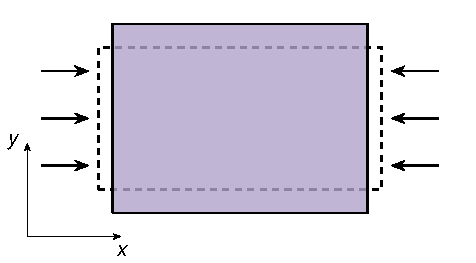
\includegraphics[width=0.6\textwidth]{Problem_1/Figs_P1/Poisson_effect.pdf}
    \caption{Hiệu ứng Poisson - vật chịu nén theo phương \(x\) sẽ giãn ra theo phương \(y\).}
    \label{fig:Poisson_effect}
\end{figure}

Để phân tích về tính chất của vật liệu chịu ảnh hưởng bởi hiệu ứng Poisson, ta sử dụng hệ số Poisson \(\nu\) được định nghĩa là giá trị âm của tỷ số biến dạng hông và biến dạng dọc trục của tấm vật liệu bị nén \footnote{Dấu âm thể hiện cho việc thông thường khi chịu nén theo một phương thì vật liệu phình theo phương còn lại.}. Điều này tức là nếu một khối vật liệu hình chữ nhật có độ dài theo trục \(x\) và trục \(y\) là \(l_x\) và \(l_y\), bị nén một đoạn \(\Delta l_x\) theo trục \(x\) và bị phình một đoạn \(\Delta l_y\) theo trục \(y\) thì hệ số Poisson \(\nu\) mô tả hiệu ứng Poisson giữa trục \(x\) và trục \(y\) được định nghĩa theo phương trình:
\begin{equation}
    \dfrac{\Delta l_x}{l_x} = - \nu \dfrac{\Delta l_y}{l_y}.
\end{equation}

Tổng quát hơn, định luật Hooke mô tả biến dạng của vật liệu đẳng hướng theo lực nén của các vật được viết lại như sau:
\begin{align*}
    \varepsilon_x &= \dfrac{1}{E} \left[ \sigma_x - \nu \left( \sigma_y + \sigma_z \right) \right], \\
    \varepsilon_y &= \dfrac{1}{E} \left[ \sigma_y - \nu \left( \sigma_z + \sigma_x \right) \right], \\
    \varepsilon_z &= \dfrac{1}{E} \left[ \sigma_z - \nu \left( \sigma_x + \sigma_y \right) \right].
\end{align*}
trong đó
\begin{itemize}
    \item \( \varepsilon_x = \Delta l_x / l_x \), \( \varepsilon_y = \Delta l_y / l_y\), \( \varepsilon_z = \Delta l_z / l_z\) lần lượt là độ biến dạng theo 3 phương \(x\), \(y\), \(z\).
    \item \(E\) là suất Young của vật liệu.
    \item \(\sigma_x\), \(\sigma_y\), \(\sigma_z\) lần lượt là ứng suất \footnote{Lực trên một đơn vị diện tích.} nén lên tấm vật liệu theo 3 phương \(x\), \(y\), \(z\).
    \item \(\nu\) là suất Poisson của vật liệu.
\end{itemize}

\ \ 

\textbf{Câu hỏi a.} Xét một khối vật liệu hình hộp chữ nhật có thể tích \(V\). Khi khối vật liệu chịu ứng suất \(p\) theo các phương, thể tích của khối hộp chữ nhật bị giảm đi \(\Delta V\). Hệ số module khối \(K\) được định nghĩa theo biểu thức
\begin{equation}
    p = - K \dfrac{\Delta V}{V}.
\end{equation}
Xác định hệ số module khối của vật liệu đó theo suất Young \(E\) và suất Poisson \(\nu\).

\ \ 

\textbf{Câu hỏi b.} Xét một vật hình hộp chữ nhật được giữ cố định độ dài theo trục \(y\) và \(z\), công thức định luật Hooke theo trục \(x\) lúc này có dạng:
\begin{equation}
    \sigma_x = f(\nu) E \varepsilon_x,
\end{equation}
với \( f(\nu) \) là một hàm phụ thuộc vào suất Poisson \(\nu\). Hãy tìm hàm \( f(\nu) \) trong bài toán trên.

\ \ 

\textbf{2. Mô hình mạng hình vuông quay}

Vật liệu auxetic là một vật liệu có thể mang lại tỷ số Poisson âm, tức là nếu như ép vật liệu này theo một phương, phương vuông góc với nó sẽ co lại theo thay vì nở ra như vật liệu thông thường. Cấu trúc mạng hình vuông quay (hình \ref{fig:Totate_processing}) là một trong những cấu trúc cơ bản nhất, là cơ sở lý thuyết cho vật liệu auxetic.

\begin{figure}[!h]
    \centering
    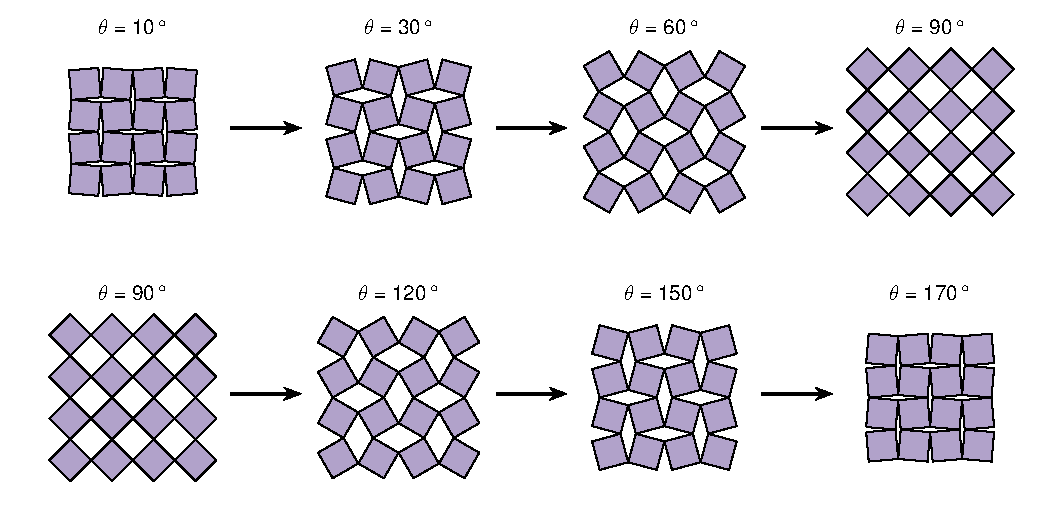
\includegraphics[width=0.96\textwidth]{Problem_1/Figs_P1/Rotate_processing.pdf}
    \caption{Quá trình giãn và co của cấu trúc mạng hình vuông quay khi tăng dần góc \(\theta\).}
    \label{fig:Totate_processing}
\end{figure}

Cấu trúc mạng hình vuông quay bao gồm các hình vuông có độ dài \(L\) ghép nối với nhau thông qua bản lề ở các góc của hình vuông, tạo thành mạng (như hình \ref{fig:Parameters_rotating_squares}). Xem rằng, các tấm hình vuông là các vật rắn không biến dạng, ta chỉ quan tâm đến các biến dạng và chuyển động trong không gian 2 chiều.

\begin{figure}[!h]
    \centering
    \begin{subfigure}{0.45\textwidth}
        \centering
        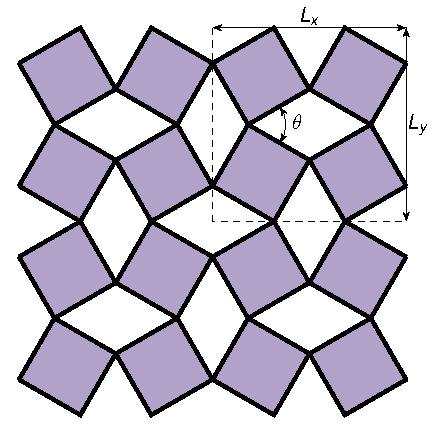
\includegraphics[width=0.9\textwidth]{Problem_1/Figs_P1/Parameters_rotating_squares.pdf}
        \caption{Các thông số hình học \(L_x\), \(L_y\) và \(\theta\) đặc trưng cho kích thước ô cơ sở.}
        \label{fig:Parameters_rotating_squares}
    \end{subfigure}
    \hspace{0.05\textwidth}
    \begin{subfigure}{0.45\textwidth}
        \centering
        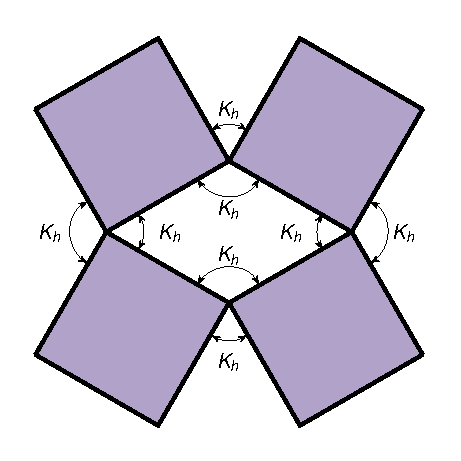
\includegraphics[width=0.95\textwidth]{Problem_1/Figs_P1/Stiffness.pdf}
        \caption{Độ cứng tại mỗi bản lề \(K_h\) trong một ô cơ sở.}
        \label{fig:Stiffness}
    \end{subfigure}
    \caption{Các thông số cấu trúc của mạng tinh thể hình vuông quay.}
\end{figure}

\ \ 

\textbf{Câu hỏi c.} Tính tỷ số Poisson của cấu trúc mạng hình vuông.

Ở thời điểm trạng thái hình học của vật được xác định bởi góc \(\theta\), xem rằng tại mỗi góc tạo bởi hai hình vuông có một moment lực xoắn gây ra bởi bản lề với độ cứng xoắn \(k_h\) (như hình \ref{fig:Stiffness}).

\ \ 

\textbf{Câu hỏi d.} Vật liệu xây dựng bởi cấu trúc mạng tinh thể hình vuông có phải vật liệu đẳng hướng trong không gian 2 chiều không? Tính suất Young từng hướng của vật liệu.
